\documentclass{beamer}

\usepackage{amsmath}

\usetheme{AnnArbor}
\usecolortheme{crane}
\usefonttheme[onlymath]{serif}

\title{Deep Learning - Foundations and Concepts}
\subtitle{Chapter 9. Regularization}
\author{nonlineark@github}
\date{\today}

\begin{document}

\begin{frame}
    \titlepage
\end{frame}

\begin{frame}
    \frametitle{Outline}
    \tableofcontents
\end{frame}

\section{Inductive Bias}

\begin{frame}
    \frametitle{Inverse problems}
    \begin{itemize}
        \item Most machine learning tasks are examples of inverse problems:
        \begin{itemize}
            \item Forward problem: Given a conditional distribution $p(t|x)$ along with a finite set of input points $\{x_{1},\hdots,x_{N}\}$, sample corresponding values $\{t_{1},\hdots,t_{N}\}$ from that distribution.
            \item Inverse problem: Infer a distribution given only a finite number of samples.
        \end{itemize}
        \item We need a way to choose a specific distribution from amongst the infinitely many possibilities. The preference for one choice over others is called inductive bias or prior knowledge:
        \begin{itemize}
            \item Small changes in the input values should lead to small changes in the output values: The sum-of-squares regularizer.
            \item When detecting objects in images, there should be translation invariance: Convolutional neural network.
            \item Additional data from a different, but related, task can be used to help determine the learnable parameters in a neural network: Transfer learning and multi-task learning.
        \end{itemize}
    \end{itemize}
\end{frame}

\begin{frame}
    \frametitle{No free lunch theorem}
    The no free lunch theorem: Every learning algorithm is as good as any other when averaged over all possible problems:
    \begin{itemize}
        \item Even very flexible neural networks contain important inductive biases, it is not possible to learn purely from data in the absence of any bias.
        \item In trying to find general-purpose learning algorithms, we are really seeking inductive biases that are appropriate to the broad classes of applications that will be encountered in practice.
        \item Inductive biases can be incorporated through:
        \begin{itemize}
            \item The form of distribution.
            \item The addition of a regularization term to the error function used during training.
            \item The training process.
        \end{itemize}
    \end{itemize}
\end{frame}

\begin{frame}
    \frametitle{Symmetry and invariance}
    \begin{itemize}
        \item In many applications of machine learning, the predictions should be unchanged under one or more transformations of the input variables:
        \begin{itemize}
            \item Translation invariance.
            \item Scale invariance.
        \end{itemize}
        \item Transformations that leave particular properties unchanged represent symmetries. The set of all transformations corresponding to a particular symmetry form a group.
    \end{itemize}
\end{frame}

\begin{frame}
    \frametitle{Symmetry and invariance}
    Efficient approaches for encouraging an adaptive model to exhibit the required invarances:
    \begin{itemize}
        \item Pre-processing: Invariances are built into a pre-processing stage by computing features of the data that are invariant under the required transformations.
        \item Regularized error function: A regularization term is added to the error function to penalize changes in the model output when the input is subject to one of the invariant transformations.
        \item Data augmentation: The training set is expanded using replicas of the training data points, transformed according to the desired invariances and carrying the same output target values as the untransformed examples.
        \item Network architecture: The invariance properties are built into the structure of a neural network through an appropriate choice of network architecture.
    \end{itemize}
\end{frame}

\begin{frame}
    \frametitle{Equivariance}
    A generalization of invariance is called equivariance in which the output of the network, instead of remaining constant when the input is transformed, is itself transformed in a specific way:
    \begin{equation*}
        \mathcal{S}(\mathcal{T}(I))=\tilde{\mathcal{T}}(\mathcal{S}(I))
    \end{equation*}
    For example:
    \begin{itemize}
        \item $\mathcal{S}$: Measures the orientation of an object within an image.
        \item $\mathcal{T}$: Rotation.
        \item $\tilde{\mathcal{T}}$: Increase or decrease the scalar orientation.
    \end{itemize}
\end{frame}

\section{Weight Decay}

\begin{frame}
    \frametitle{Weight decay}
    \begin{itemize}
        \item The simplest regularizer comprises the sum of the squares of the model parameters: $\tilde{E}(w)=E(w)+\frac{\lambda}{2}w^{T}w$.
        \item The sum-of-squares regularizer is known as weight decay because it encourages weight values to decay towards zero.
        \item The sum-of-squares regularizer can be interpreted as the negative logarithm of a zero-mean Gaussian prior distribution over the weight vector $w$, which is a way to include prior knowledge into the model training process.
        \item It is trivial to evaluate its derivatives for use in gradient descent training: $\nabla\tilde{E}(w)=\nabla{}E(w)+\lambda{}w$.
    \end{itemize}
\end{frame}

\begin{frame}
    \frametitle{Weight decay}
    Consider a two-dimensional parameter space along with a sum-of-squares error function $E(w)$:
    \begin{itemize}
        \item The effect of the regularization term is to shrink the magnitudes of the weight parameters.
        \item The effect is much larger for the parameter corresponds to the smaller eigenvalue (here $w_{1}$) compared to that of the parameter corresponds to the larger eigenvalue (here $w_{2}$).
        \item The effective number of parameters is the number that remain active after regularization.
        \item Controlling model complexity by regularization has similarities to controlling model complexity by limiting the number of parameters:
        \begin{itemize}
            \item $\lambda\to\infty$: The effective number of parameters is zero.
            \item $\lambda=0$: The effective number of parameters equals the total number of parameters in the model.
        \end{itemize}
    \end{itemize}
\end{frame}

\begin{frame}
    \frametitle{Weight decay}
    \begin{figure}
        \caption{Effect of a quadratic regularizer}
        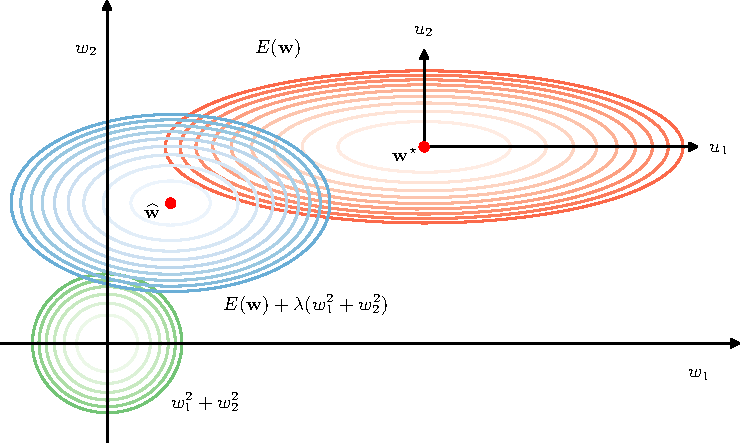
\includegraphics[height=0.7\textheight]{Figure_3.pdf}
    \end{figure}
\end{frame}

\begin{frame}
    \frametitle{Consistent regularizers}
    Consider a two-layer network of the form:
    \begin{align*}
        z_{j}&=h(\sum_{i}w_{ji}x_{i}+w_{j0})&y_{k}&=\sum_{j}w_{kj}z_{j}+w_{k0}
    \end{align*}
    Observe that linear transformations of the input data or output variables can be balanced by making a corresponding linear transformation of the weights and biases so that the mapping performed by the network is unchanged:
    \begin{align*}
        x_{i}&\to\tilde{x}_{i}=ax_{i}+b&y_{k}&\to\tilde{y}_{k}=cy_{k}+d \\
        w_{ji}&\to\tilde{w}_{ji}=\frac{1}{a}w_{ji}&w_{kj}&\to\tilde{w}_{kj}=cw_{kj} \\
        w_{j0}&\to\tilde{w}_{j0}=w_{j0}-\frac{b}{a}\sum_{i}w_{ji}&w_{k0}&\to\tilde{w}_{k0}=cw_{k0}+d
    \end{align*}
\end{frame}

\begin{frame}
    \frametitle{Consistent regularizers}
    Clearly, the simple sum-of-squares weight decay does not have this consistency. We look for a regularizer that is invariant to re-scaling of the weights and to shifts of the biases:
    \begin{equation*}
        \frac{\lambda_{1}}{2}\sum_{w\in\mathcal{W}_{1}}w^{2}+\frac{\lambda_{2}}{2}\sum_{w\in\mathcal{W}_{2}}w^{2}
    \end{equation*}
    where $\mathcal{W}_{1}$ denotes the set of weights in the first layer, $\mathcal{W}_{2}$ denotes the set of weights in the second layer. Because biases are excluded from the summations, the prior distribution over the parameters is improper:
    \begin{equation*}
        p(w;\lambda_{1},\lambda_{2})\propto\exp(-\frac{\lambda_{1}}{2}\sum_{w\in\mathcal{W}_{1}}w^{2}-\frac{\lambda_{2}}{2}\sum_{w\in\mathcal{W}_{2}}w^{2})
    \end{equation*}
    It is therefore common to include separate priors for the biases (which then break the shift invariance) that have their own hyperparameters.
\end{frame}

\begin{frame}
    \frametitle{Consistent regularizers}
    More generally, we can consider regularizers in which the weights are divided into any number of groups $\mathcal{W}_{k}$ so that:
    \begin{equation*}
        \Omega(w)=\frac{1}{2}\sum_{k}\lambda_{k}||w||_{k}^{2}=\frac{1}{2}\sum_{k}\lambda_{k}\sum_{w\in\mathcal{W}_{k}}w^{2}
    \end{equation*}
    For example, we could use a different regularizer for each layer in a multilayer network.
\end{frame}

\begin{frame}
    \frametitle{Generalized weight decay}
    Generalization of the simple quadratic regularizer:
    \begin{equation*}
        \Omega(w)=\frac{\lambda}{2}\sum_{m=1}^{M}|w_{m}|^{q}
    \end{equation*}
    where:
    \begin{itemize}
        \item $q=2$ corresponds to the quadratic regularizer.
        \item $q=1$ is known as a lasso. For quadratic error functions, it has the property that if $\lambda$ is sufficiently large, some of the coefficients $w_{j}$ are driven to zero, leading to a sparse model.
    \end{itemize}
\end{frame}

\begin{frame}
    \frametitle{Generalized weight decay}
    \begin{figure}
        \caption{Lasso vs. quadratic regularizer}
        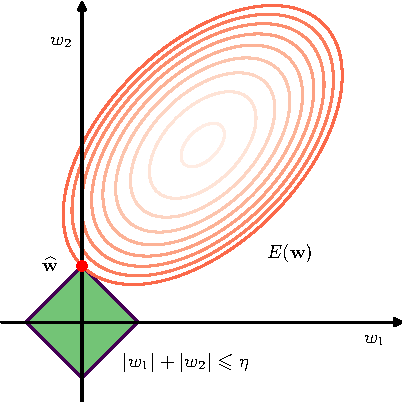
\includegraphics[width=0.4\textwidth]{Figure_6_a.pdf}
        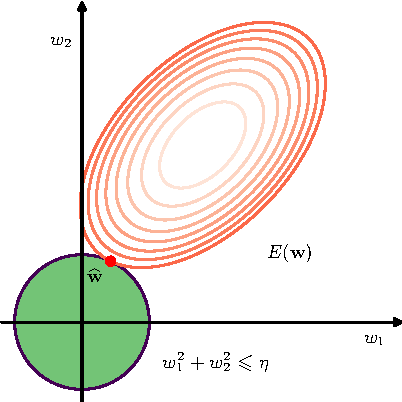
\includegraphics[width=0.4\textwidth]{Figure_6_b.pdf}
    \end{figure}
\end{frame}

\section{Learning Curves}

\begin{frame}
    \frametitle{Learning curves}
    During optimization of the error function through gradient descent:
    \begin{itemize}
        \item The training error typically decreases as the model parameters are updated.
        \item The error for validation data may be non-monotonic.
    \end{itemize}
    This behavior can be visualized using learning curves, which provide insight into the progress of training and also offer a practical methodology for controlling the effective model complexity.
\end{frame}

\begin{frame}
    \frametitle{Early stopping}
    To obtain a network with good generalization performance, training should be stopped at the point of smallest error with respect to the validation data set.
    \begin{figure}
        \caption{An illustration of the behavior of training set error and validation set error during a typical training session}
        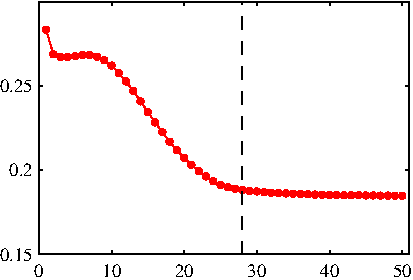
\includegraphics[width=0.4\textwidth]{Figure_7_a.pdf}
        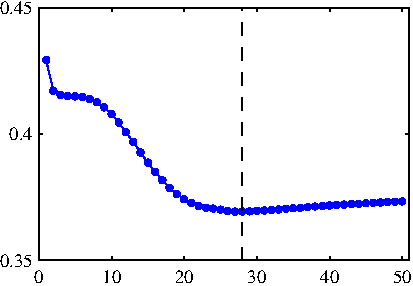
\includegraphics[width=0.4\textwidth]{Figure_7_b.pdf}
    \end{figure}
\end{frame}

\begin{frame}
    \frametitle{Early stopping}
    This behavior of the learning curves is sometimes explained qualitatively in terms of the effective number of parameters in the network:
    \begin{itemize}
        \item This number starts out small and grows during training.
        \item Early stopping is a way to limit the effective network complexity.
    \end{itemize}
    \begin{figure}
        \caption{Early stopping can give similar results to weight decay for a quadratic error function}
        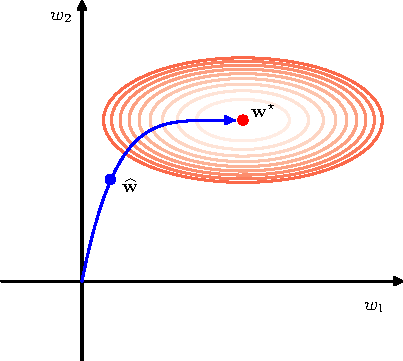
\includegraphics[height=0.4\textheight]{Figure_8.pdf}
    \end{figure}
\end{frame}

\begin{frame}
    \frametitle{Double descent}
    Modern deep neural networks defeat the conventional belief:
    \begin{itemize}
        \item Conventional belief: The number of parameters in the model needs to be limited according to the size of the data set and that for a given training data set, very large models are expected to have poor performance.
        \item The general wisdom in the deep learning community is that bigger models are better.
    \end{itemize}
\end{frame}

\begin{frame}
    \frametitle{Double descent}
    \begin{figure}
        \caption{Plot of training set and test set errors for a large neural network model versus the complexity of the model}
        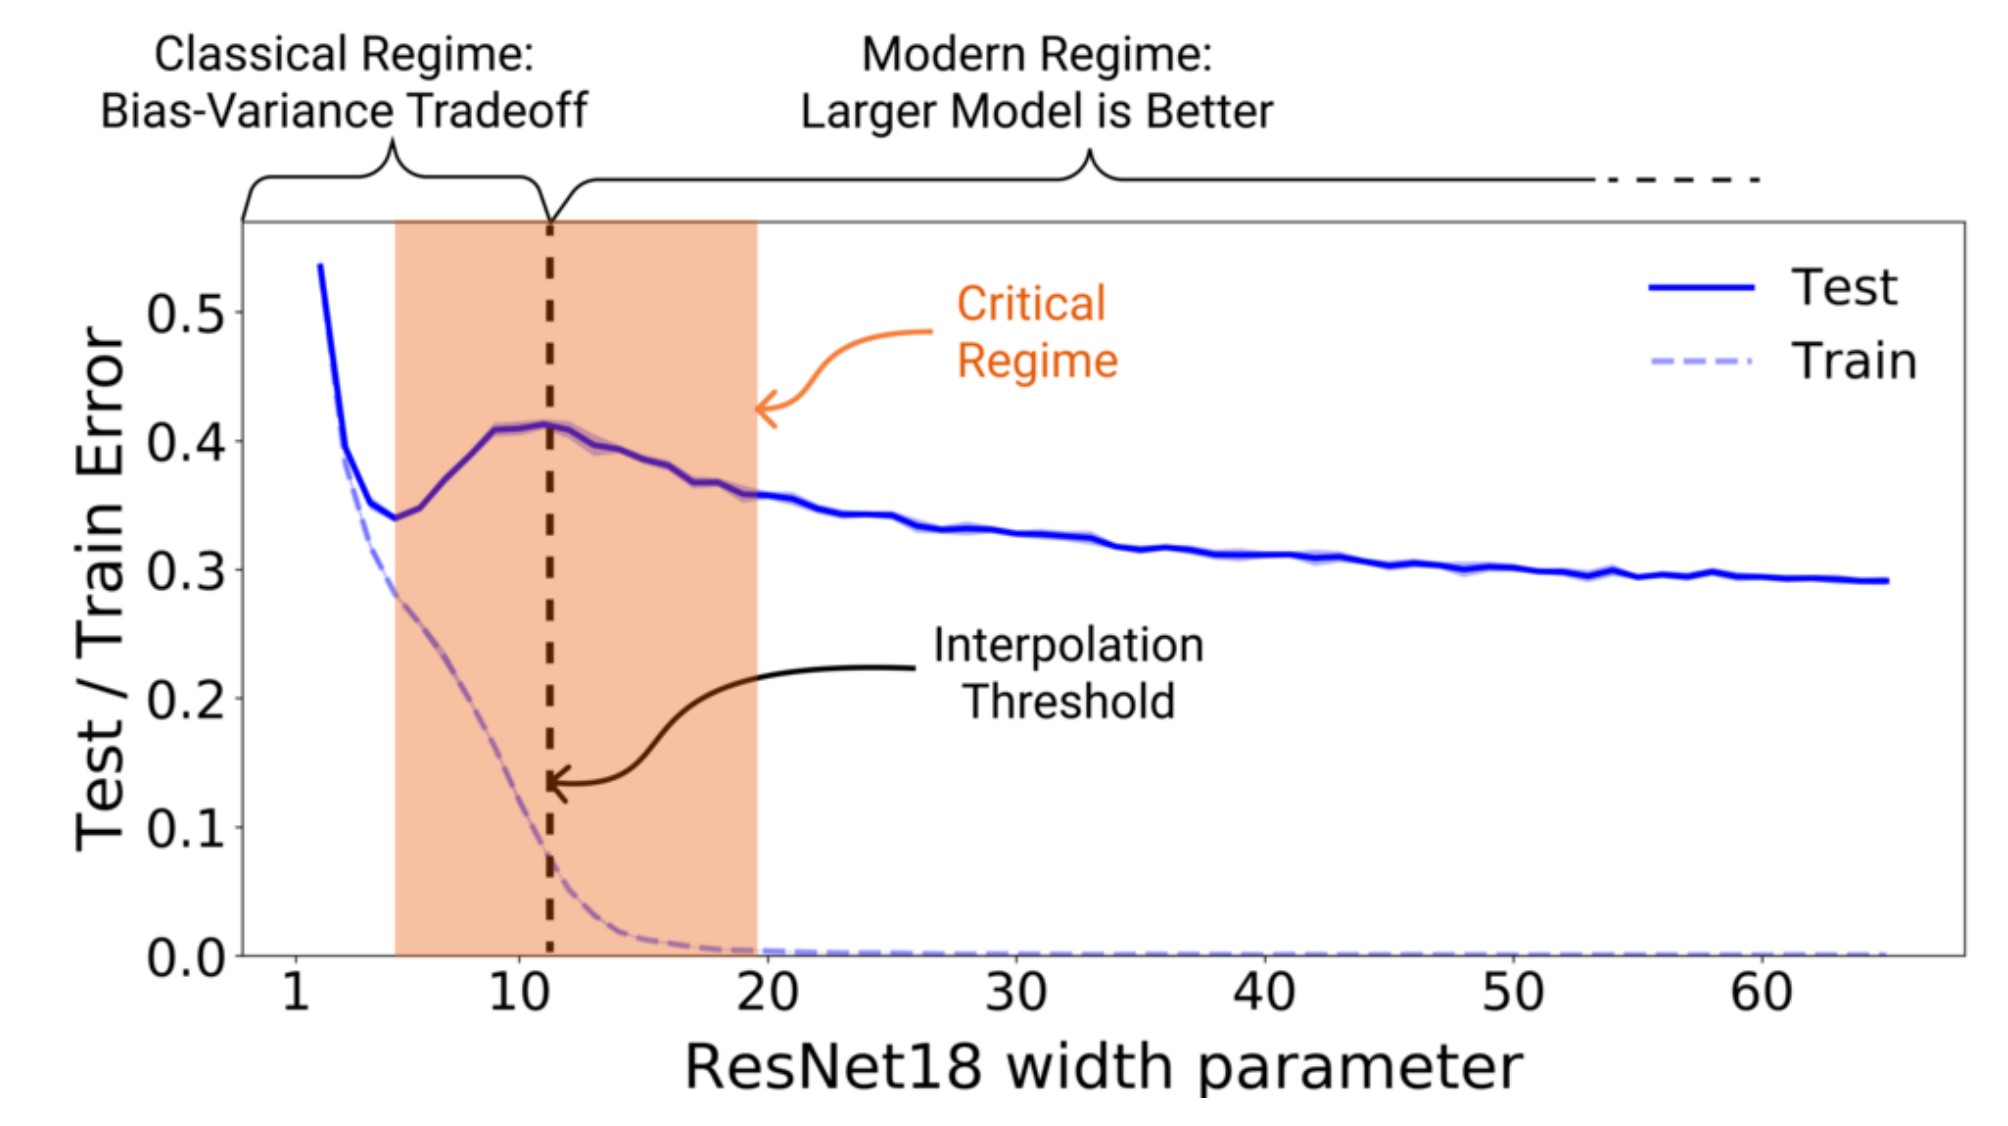
\includegraphics[height=0.6\textheight]{Figure_9.jpg}
    \end{figure}
\end{frame}

\begin{frame}
    \frametitle{Double descent}
    The surprising behavior exhibits two different regimes of model fitting:
    \begin{itemize}
        \item The classical bias-variance trade-off for small to medium complexity.
        \item Followed by a further reduction in test set error as we enter a regime of very large models.
        \item The transition between the two regimes occurs roughly when the model is complex enough that the model is able to fit the training data exactly:
        \begin{itemize}
            \item Effective model complexity: The maximum size of training data set on which a model can achieve zero training error.
            \item Double descent arises when the effective model complexity exceeds the number of data points in the training set.
            \item It is possible to operate in a regime where increasing the size of the training data set could actually reduce performance.
        \end{itemize}
    \end{itemize}
\end{frame}

\end{document}